\documentclass{article}
\usepackage{graphicx} % Required for inserting images
\usepackage{natbib} % For \citep and other citation commands
\usepackage{float} % For [H] float placement
\usepackage{amsmath} % For \text in math mode

\title{Solar Panel Tech Description}
\author{Dana Golden and Yiyi Zhou}
\date{March 2026}

\begin{document}

\maketitle

\section{Supply Chain: Monocrystalline Silicon Panels}
 
The production of monocrystalline silicon (c-Si) photovoltaic modules proceeds through a series of discrete, geographically dispersed batch processes \citep{Powell2012, Woodhouse2019}. The first stage involves refining raw quartz into high-purity polysilicon, typically via the Siemens process, in which a silicon--hydrogen--chlorine gas compound is decomposed onto heated silicon filaments \citep{DOE_manufacturing}.

The resulting polysilicon feedstock is then melted and drawn into a single-crystal cylindrical ingot using the Czochralski (Cz) method, an energy-intensive process requiring sustained temperatures above 1414\textdegree{}C \citep{Czochralski1918, Costa2017}. Once the ingot is grown, it is sawn into wafers---currently in the 150--180~$\mu$m thickness range---using diamond wire cutting \citep{ITRPV2024}. This wafering step entails substantial material loss, referred to as kerf loss, which remains on the order of 60--110~$\mu$m per cut despite ongoing improvements in wire diameter \citep{ITRPV2024}.
 
The resulting wafers then undergo cell fabrication, in which they are doped with phosphorus or boron to form a p--n junction, coated with anti-reflective layers (typically silicon nitride), and metallized with screen-printed silver gridlines for current collection \citep{Powell2012, Woodhouse2019}. Finally, individual cells are soldered into strings, encapsulated in ethylene-vinyl acetate (EVA), laminated beneath a glass front sheet, and fitted with an aluminum frame and junction box to produce the finished module \citep{DOE_manufacturing}.
 
\section{Supply Chain: Thin-Film Modules}
 
In contrast to the discrete, multi-facility production chain of c-Si panels, thin-film manufacturing---exemplified by cadmium telluride (CdTe) and copper indium gallium selenide (CIGS) technologies---follows a highly integrated, continuous-flow paradigm in which the entire module is fabricated from substrate to finished product within a single facility \citep{DOE_manufacturing, Fthenakis2008}. This architecture eliminates the need for separate ingot growth, wafering, and individual cell fabrication. Instead, monolithic interconnection is achieved through sequential laser scribing of the continuous deposited film, which patterns the sheet into series-connected cells without manual wiring \citep{Amin2017}.
  
The primary inputs to thin-film production are a substrate and semiconductor precursor materials. The substrate is typically a sheet of soda-lime glass or, in some configurations, a flexible polymer \citep{Fthenakis2011}. Deposition of the active layers proceeds via high-throughput techniques such as close-spaced sublimation (CSS) for CdTe or co-evaporation and sputtering for CIGS, along with transparent conductive oxide (TCO) front contacts deposited by sputtering or chemical vapor deposition (CVD) \citep{Amin2017, Bonnet2002}.

Because the active semiconductor layer in thin-film modules is typically only 1-10~$\mu$m thick \citep{Amin2017}, the material and embodied energy requirements per unit area are substantially lower than those of c-Si production, as reflected in shorter energy payback times \citep{Fthenakis2011, Raugei2007}.
 
\section{Differences in Cost Structures}
 
The cost structures of thin-film and c-Si manufacturing differ markedly in their relative weighting of fixed and variable components \citep{Powell2012, Powell2013}. Thin-film production entails large upfront capital expenditures for specialized vacuum deposition chambers, laser scribing equipment, and highly automated conveyance systems. However, because the active layers require minimal material per module, marginal production costs are low. This cost profile heavily weights thin-film economics toward fixed costs, requiring manufacturers to operate at high capacity utilization rates to amortize their facility investments effectively \citep{Goodrich2013}.
 
Monocrystalline silicon production, by contrast, is characterized by comparatively high variable costs. The energy-intensive Czochralski crystal growth process, the consumption of high-purity polysilicon feedstock, and the reliance on silver paste for metallization and aluminum for framing collectively ensure that the marginal cost of each additional module remains substantial \citep{Powell2012, Woodhouse2019}. Consequently, c-Si manufacturers face greater exposure to input price volatility and supply chain disruptions affecting commodity markets for polysilicon, silver, and aluminum \citep{ITRPV2024}.

Figure \ref{fig:Costs} presents the breakeven decision from a manufacturing cost standpoint between producing each of the different technologies. c-Si is a significantly cheaper technology to produce for lower capacity levels, but beyond a certain production level thin-film dominates. This trend may explain why learning-by-doing effects are so large for c-Si panels as high variable costs are better suited to process improvements. The relationship may also provide clues as to why input subsidies had such a differential effect on firm technology choice. If thin-film firms do not reach critical capacity, they remain higher cost providers and thus out of the market. By subsidizing c-Si early, the Chinese government may have created barriers to reaching critical scale for CdTe manufacturing.

\begin{figure}[H]
    \centering
    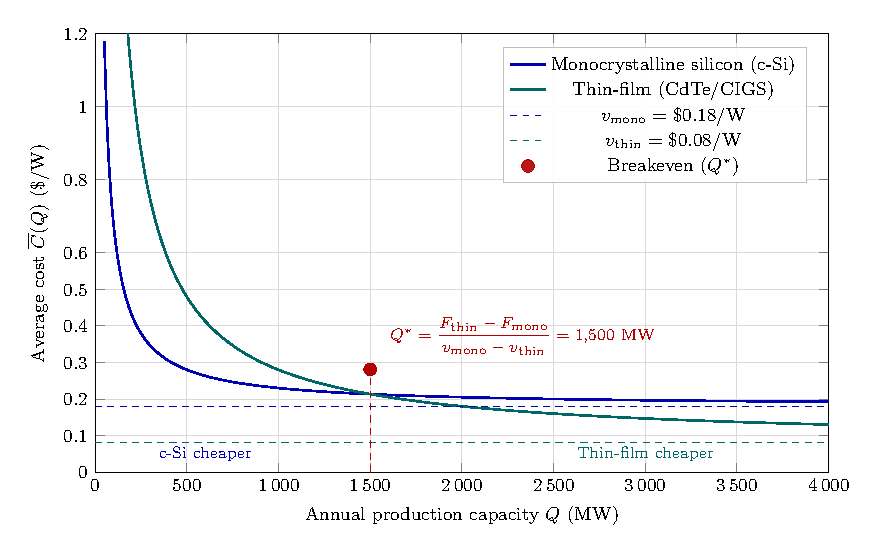
\includegraphics[width=0.5\linewidth]{images/lcoe_crossover.pdf}
    \caption{Thin-film is cheaper beyond a certain level of production.}
    \label{fig:Costs}
\end{figure}

\section{Supply Chain Map}

The supply chain map shown in Figure \ref{fig:SupplyChainMap} provides a visualization of the differences between the supply chains thin-film and monocrystalline panels. While c-Si panels are produced by a long multi-echelon supply chain that includes many materials prior to reaching the manufacturing stage, due to the less intense nature of the material inputs and the more coordinated manufacturing process, CdTe panels tend to be more vertically integrated with a shorter more concentrated supply chain.

One very important additional note to make is that there has been a strong trend of reusing solar manufacturing facilities in China for other manufactured products as prices fall to the floor. It is significantly easier to re-purpose c-Si facilities than CdTe facilities both because c-Si facilities are less specialized and because China has a burgeoning power electronics ecosystem in need of c-Si manufacturing capacity. This increases scrap value of c-Si firms and makes monocrystalline manufacturing slightly more desirable for firms. It also increases the desirability of monocrystalline manufacturing facilities to the provincial and national government by decreasing the cost of firm exit.

\begin{figure}[H]
    \centering
    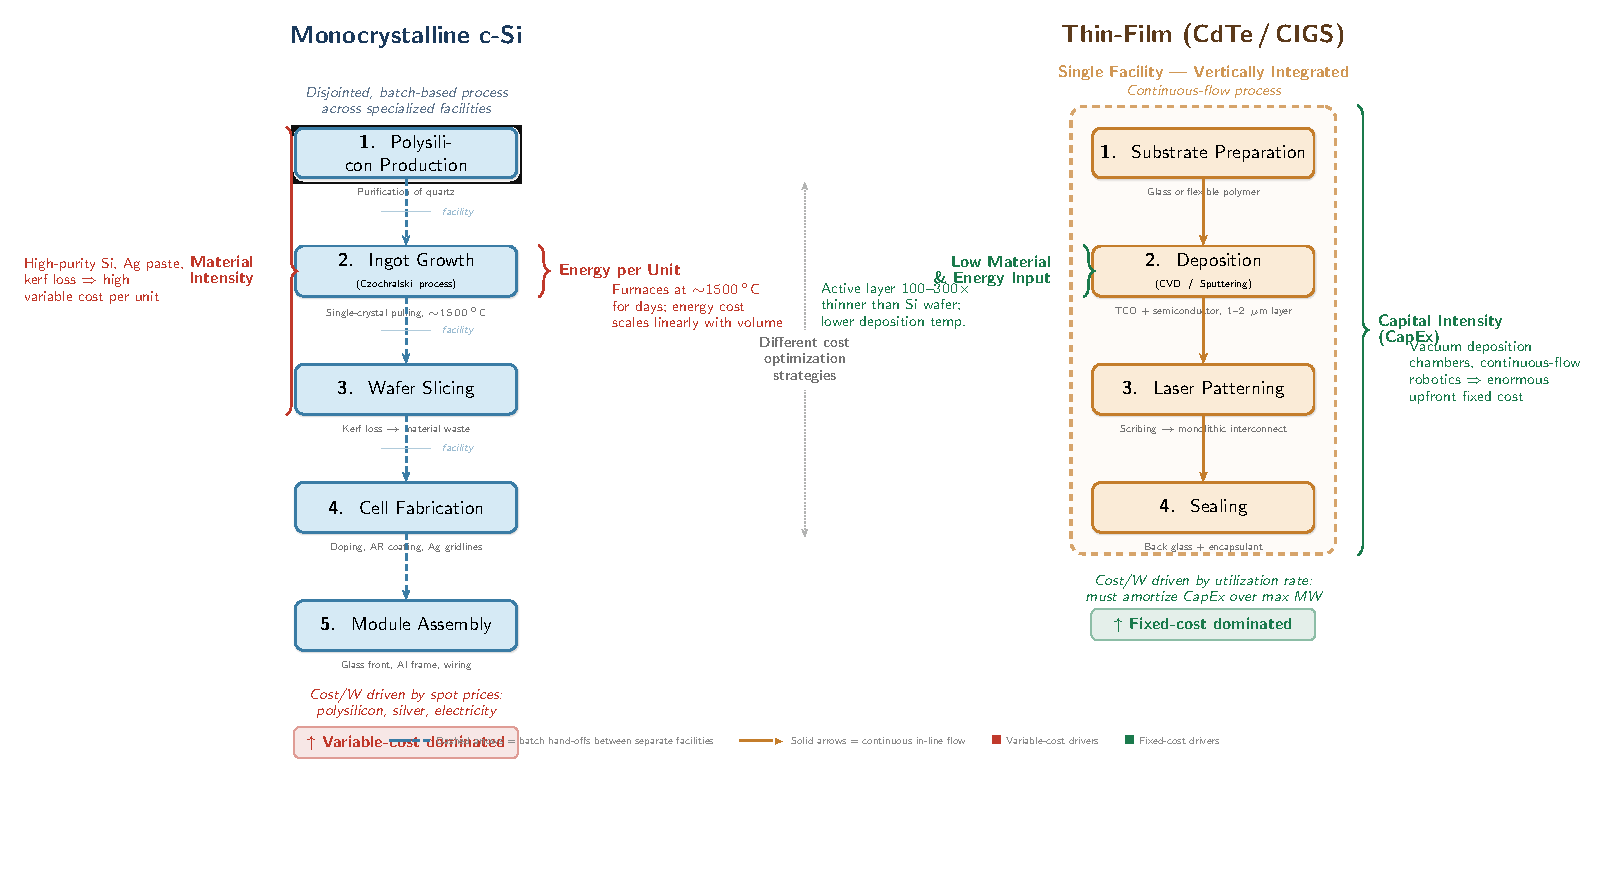
\includegraphics[width=\linewidth]{images/supply_chain_figure.pdf}
    \caption{Differences between production and cost structures by product type.}
    \label{fig:SupplyChainMap}
\end{figure}

\section{Differences in Market Demand}

While the preceding sections characterize differences in production processes and cost structures, the two technologies also present distinct performance profiles to the power system operators, project developers, and end consumers who procure them. The relevant dimensions include conversion efficiency (and the land area it implies), degradation over the module lifetime, and sensitivity to operating temperature.
 
\subsection{Conversion Efficiency and Area Requirements}
 
The most salient demand-side distinction is module-level conversion efficiency. Commercial monocrystalline silicon modules currently achieve efficiencies in the range of 20--23\%, with the best laboratory cells reaching 26.8\% \citep{Green2024}. CdTe thin-film modules, the dominant thin-film technology, have improved substantially but remain lower, with commercial modules in the 18--20\% range and a record research-cell efficiency of 22.4\% \citep{Green2024, NREL_CdTe2025}. The gap is narrower than it once was, and fleet-average CdTe module efficiencies have historically tracked within a reasonable margin of monocrystalline silicon \citep{NREL_CdTe2025}, but the difference remains consequential for land-constrained applications.
 
Because lower-efficiency modules require more panel area to achieve a given nameplate capacity, technology choice directly affects land-use intensity at the utility scale. For a fixed power target, a thin-film installation will occupy a larger footprint than a c-Si installation, all else equal \citep{Ong2013, Bolinger2022}. This distinction is less material in settings with abundant inexpensive land---such as desert utility-scale deployments---but becomes a binding constraint for rooftop, commercial, and building-integrated applications where available area is fixed \citep{EIA2018}.
 
\subsection{Degradation}
 
All photovoltaic modules experience gradual power output decline over their operational lifetime, but degradation rates differ across technologies. A comprehensive meta-analysis by \citet{Jordan2016}, aggregating more than 11{,}000 field-measured degradation rates across 40 countries, found median annual degradation rates for crystalline silicon technologies in the range of 0.5--0.6\%/year. An earlier review by \citet{Jordan2013} documented a median rate of approximately 0.5\%/year across nearly 2{,}000 observations spanning four decades of field exposure. Thin-film technologies, particularly early-generation amorphous silicon, have historically exhibited higher degradation rates, though more recent CdTe and CIGS modules have shown improved stability \citep{Jordan2016}. The practical implication is that c-Si modules are more likely to retain a higher fraction of their initial rated output over a 25--30 year project life, which affects lifetime energy yield and the levelized cost of energy (LCOE).
 
\subsection{Temperature Sensitivity}
 
Photovoltaic power output declines as cell temperature rises above the standard test condition of 25\textdegree{}C, a relationship captured by the temperature coefficient of power ($\beta$). Crystalline silicon modules exhibit temperature coefficients typically in the range of $-0.3$ to $-0.5$\%/\textdegree{}C, whereas CdTe thin-film modules generally have more favorable coefficients around $-0.2$\%/\textdegree{}C \citep{Skoplaki2009}. This difference is nontrivial in hot climates: at an operating cell temperature of 65\textdegree{}C (i.e., 40\textdegree{}C above STC), a c-Si module with $\beta = -0.4$\%/\textdegree{}C loses approximately 16\% of its rated output, whereas a CdTe module with $\beta = -0.2$\%/\textdegree{}C loses only about 8\%. In desert and tropical installations where sustained high temperatures are common, the superior thermal response of thin-film modules partially offsets their lower nominal efficiency, narrowing the effective energy yield gap between the two technologies \citep{Alqahtani2022}.
 
\subsection{Implications for Technology Selection}
 
Together, these demand-side characteristics create a differentiated value proposition for each technology. Monocrystalline silicon's higher efficiency and lower degradation make it the default choice where land area is constrained, where rooftop or distributed deployment is intended, or where long project lifetimes place a premium on sustained output. 

Thin-film CdTe modules, by contrast, offer advantages in hot-climate utility-scale deployments where land is inexpensive, temperature-related derating is a significant concern, and the lower embodied energy and simpler manufacturing process may translate into lower module costs and faster energy payback \citep{Fthenakis2011, NREL_CdTe2025}.

The competitive dynamics between the two technologies are further shaped by the rapid pace of efficiency improvements in both camps, particularly as c-Si manufacturers transition to advanced cell architectures such as TOPCon and heterojunction designs \citep{ITRPV2024}. c-Si panels tend to be used in larger systems creating a breakeven point beyond which monocrystalline panels are preferred on the demand side. Figure \ref{fig:CostsUtility} illustrates this breakeven choice between the system types for consumers of power generation systems.

\begin{figure}[H]
    \centering
    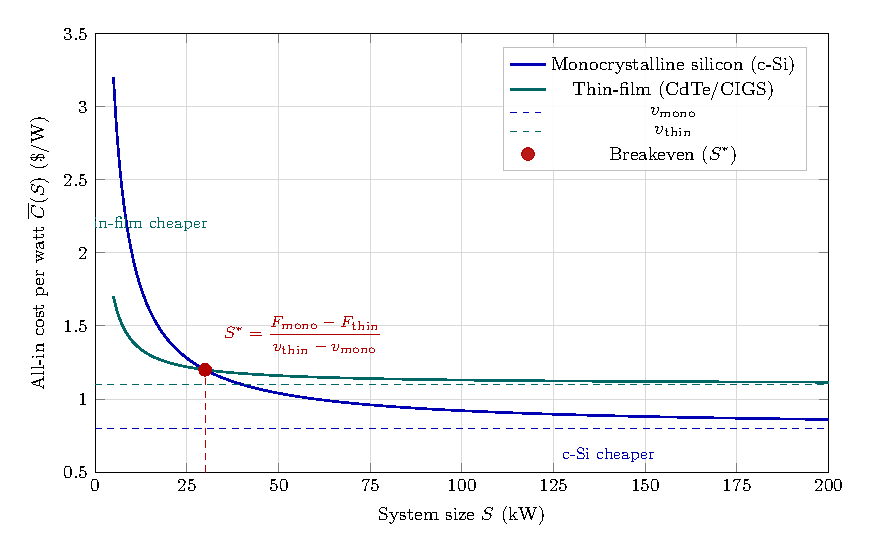
\includegraphics[width=0.5\linewidth]{images/ConsunmerProblem.pdf}
    \caption{Monocrystalline preferred for utility-scale systems.}
    \label{fig:CostsUtility}
\end{figure}

\section{Lifecycle Analysis}
 
The lifecycle environmental profile of photovoltaic technologies varies substantially across cell architectures, and the comparison between crystalline silicon (c-Si) and cadmium telluride (CdTe) thin-film panels is especially relevant for evaluating the Chinese solar industry's global welfare impact. Chinese manufacturers overwhelmingly produce c-Si panels, while the leading CdTe producer---First Solar, headquartered in the United States---represents a fundamentally different technological pathway with distinct lifecycle characteristics. This section reviews the evidence across four lifecycle stages: manufacturing energy use, energy payback, greenhouse gas emissions, and end-of-life management. Figure \ref{fig:LifecycleViz} provides a visualization of how the different processes for module creation impact lifecycle considerations.

\begin{figure}
    \centering
    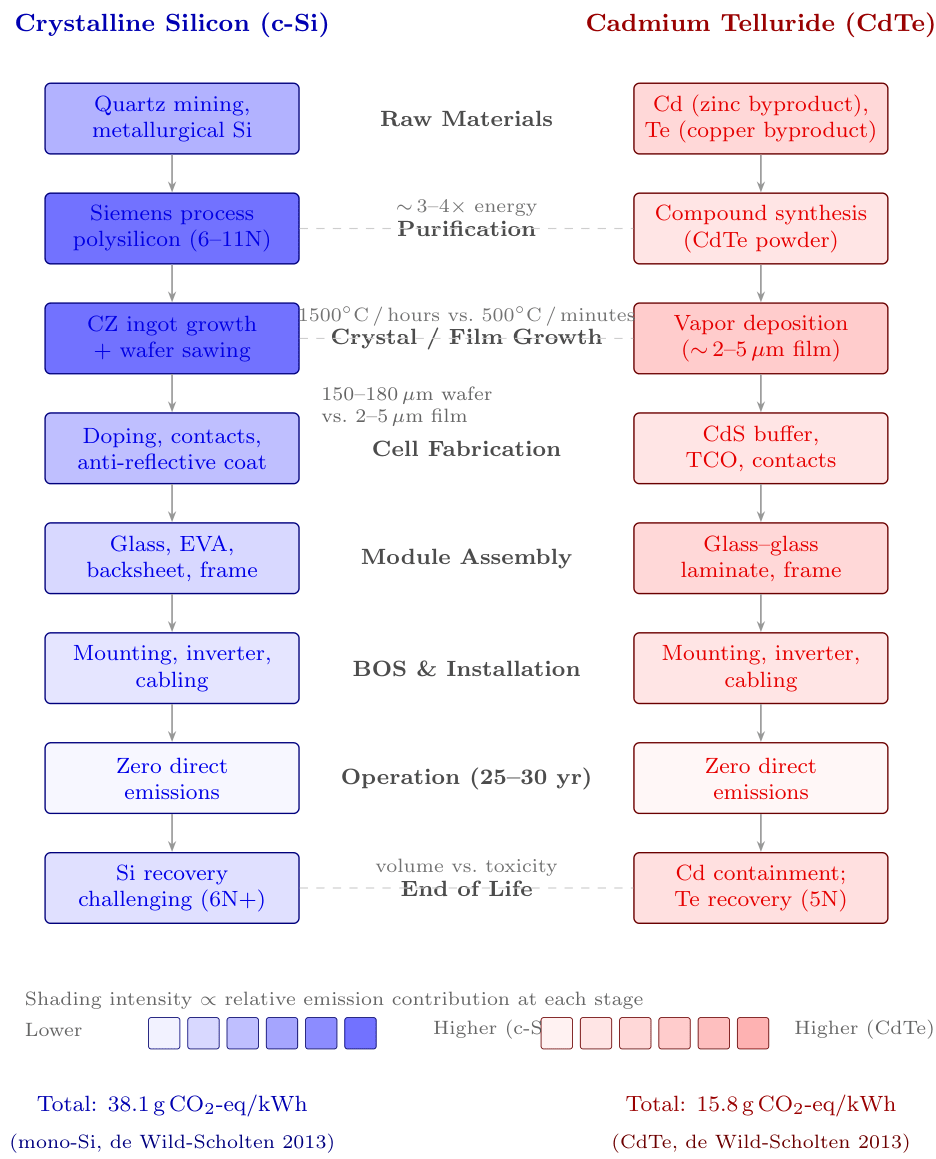
\includegraphics[width=0.5\linewidth]{images/Solar Panel Lifecycle.png}
    \caption{Lifecylce analysis visualized.}
    \label{fig:LifecycleViz}
\end{figure}
 
\subsection{Manufacturing Energy Intensity}
 
The manufacturing energy requirements of c-Si and CdTe panels differ by roughly an order of magnitude at the module level. Crystalline silicon production involves energy-intensive silicon purification (via the Siemens process), ingot crystallization, and wafer sawing. For monocrystalline panels, the Czochralski (CZ) ingot growth process operates at approximately 1500$^\circ$C for extended periods, adding a further energy penalty beyond that of multicrystalline directional solidification \citep{zagtouli2023}. \citet{fthenakiskim2011} report lifecycle primary energy consumption on the order of 3700--4900~MJ/m$^2$ for c-Si modules (depending on mono- vs.\ multi-Si and the polysilicon production route), compared to approximately 1200~MJ/m$^2$ for CdTe modules based on actual production data from First Solar's 25~MW$_\text{p}$ plant.
 
This differential reflects a basic physical distinction. CdTe thin-film deposition processes---typically vapor transport or close-space sublimation at 450--600$^\circ$C---require far less thermal energy than the high-temperature melt processes central to c-Si wafer production. The semiconductor layer in a CdTe module is only a few microns thick, whereas c-Si wafers are typically 150--180~$\mu$m, implying orders-of-magnitude less active material per unit area. The tradeoff is efficiency: modern mono-Si PERC cells achieve 20--22\% module efficiency versus 18--19\% for the latest CdTe modules, meaning more CdTe panel area is needed per unit of installed capacity \citep{smith2024nrel}.
 
A critical mediating variable is the carbon intensity of the electricity grid powering manufacturing. \citet{dewild2013} show that shifting c-Si production to China increases lifecycle carbon footprints by a factor of 1.3--2.1 relative to European production, depending on manufacturing electricity intensity. Because CdTe manufacturing is concentrated in less carbon-intensive grid regions (First Solar's primary facilities are in the United States, Malaysia, and Vietnam), the manufacturing carbon differential between the two technologies is even wider than the energy differential alone would suggest.
 
\subsection{Energy Payback Time}
 
Energy payback time (EPBT)---the period required for a PV system to generate the energy equivalent consumed in its production---is where CdTe's manufacturing advantage translates most directly into lifecycle performance. Among the five major commercial PV technologies reviewed by \citet{peng2013}, CdTe exhibits the shortest EPBT, primarily due to its low lifecycle energy requirement combined with competitive conversion efficiency for a thin-film technology. The same review finds that mono-Si systems exhibit the longest EPBT among commercial technologies, driven by the energy intensity of CZ ingot growth and silicon purification.
 
For specific estimates, \citet{fthenakiskim2011} report an EPBT of 1.1 years for ground-mounted CdTe PV systems under average U.S. insolation (1800~kWh/m$^2$/yr), including balance-of-system (BOS) components. \citet{fthenakiskim2005} provide a more disaggregated accounting: CdTe module EPBT of 0.75 years, rising to 1.2 years with optimized ground-mounted BOS. By comparison, mono-Si EPBTs in the same era were 1.7--2.7 years \citep{peng2013}, and multi-Si EPBTs were 1.2--2.0 years under comparable conditions \citep{fthenakiskim2011}.
 
These figures have shifted substantially for c-Si in recent years as manufacturing has scaled and silicon utilization has improved. The most recent NREL assessment of U.S. utility-scale mono-Si systems reports EPBT of 0.5--1.2 years, with a benchmark of 0.6 years for a 100~MW$_\text{dc}$ system using 20.3\%-efficient PERC modules on single-axis trackers \citep{smith2024nrel}. The convergence between c-Si and CdTe EPBT estimates in recent literature reflects both genuine improvements in c-Si manufacturing efficiency and the fact that CdTe efficiency has not risen as rapidly as c-Si over the past decade. Nevertheless, \citet{dewild2013} report that CdTe retains the lowest EPBT (0.68 years) among the six commercial technologies assessed under standardized Southern European conditions, compared to 1.96 years for mono-Si, 1.24 years for multi-Si, and 0.92 years for micromorph silicon.
 
\subsection{Lifecycle Greenhouse Gas Emissions}
 
The GHG emission comparison reinforces CdTe's lifecycle advantage but reveals important sensitivity to manufacturing location and grid assumptions. \citet{fthenakis2008} provide a comprehensive decomposition across four PV technologies and find that CdTe emits the fewest GHGs per kWh, primarily because thin-film manufacturing requires less energy and consequently less fossil-fuel-derived electricity. Lifecycle cadmium emissions from CdTe PV are paradoxically lower than from c-Si PV: the former uses less energy overall, and indirect Cd emissions from electricity consumption dominate direct emissions from the CdTe semiconductor itself \citep{fthenakis2008}.
 
Specific emission estimates have declined over time for both technologies. \citet{dewild2013} report lifecycle GHG emissions of 15.8~g~CO$_2$-eq/kWh for CdTe, compared to 38.1~g~CO$_2$-eq/kWh for mono-Si and 27.2~g~CO$_2$-eq/kWh for multi-Si, under baseline assumptions (European production with hydropower-sourced polysilicon, Southern European insolation of 1700~kWh/m$^2$/yr). The latest NREL assessment finds 10--36~g~CO$_2$-eq/kWh for U.S. utility-scale mono-Si systems, depending on supply chain and location \citep{smith2024nrel}. The NREL Harmonization Project, reviewing over 400 published c-Si LCA estimates, reports a harmonized median around 45~g~CO$_2$-eq/kWh for the studies available at the time of review \citep{hsu2012}, while the companion thin-film harmonization finds substantially lower medians for CdTe \citep{kim2012thinfilm}.
 
Critically, the GHG differential widens when manufacturing occurs in coal-intensive regions. Chinese c-Si production, which dominates global supply, embeds the carbon intensity of China's electricity mix at the point and time of manufacture. This creates a structural lifecycle penalty for Chinese c-Si relative to CdTe modules manufactured in regions with less carbon-intensive grids. For policymakers evaluating embodied carbon in traded PV modules, this supply-chain geography matters as much as the underlying technology choice.
 
\subsection{End-of-Life Management}
 
The two technologies present distinct end-of-life challenges. Crystalline silicon modules are composed of approximately 70\% glass, 18\% aluminum (frame), 5\% silicon, and smaller fractions of copper, silver, and polymeric encapsulants by mass \citep{recyclingreview2024}. The EU's WEEE Directive mandates 85\% collection and 80\% recycling by mass for PV panels \citep{weee2012}, and current European industrial processes for c-Si exceed these targets: the Veolia facility in Rousset, France achieves approximately 94.7\% mass recovery \citep{pvcycle2020}. However, recovery of solar-grade silicon remains the critical bottleneck. Silicon wafer production requires purity of 99.9999\% (6N) or higher, and recovered silicon is typically contaminated with dopants, requiring energy-intensive re-refining that partially negates the lifecycle energy savings from recycling \citep{cas2024}.
 
CdTe recycling follows a fundamentally different pathway, driven by the imperative of containing cadmium---a known carcinogen---and recovering tellurium, a scarce byproduct of copper mining. First Solar operates the only large-scale, vertically integrated CdTe recycling program, with facilities in the United States, Germany, and Malaysia. The process combines mechanical shredding, chemical leaching, and precipitation to recover approximately 90\% of glass and 95\% of semiconductor material \citep{sinha2012, firstsolar2024sustainability}. First Solar has demonstrated refining of recovered CdTe to 99.999\% (5N) purity, suitable for reuse in new modules \citep{firstsolarreview2015}. 

This closed-loop capability is significant: because tellurium supply could become a constraint if CdTe deployment scales substantially---demand projections suggest a potential sevenfold increase by 2040 \citep{CdTewaste2024}---the ability to recycle semiconductor material back into production at solar-grade purity creates a more circular material flow than is currently achievable for c-Si.
 
However, outside of First Solar's proprietary program, CdTe end-of-life modules are primarily landfilled in the United States, as recycling remains more expensive than disposal under current regulatory and market conditions \citep{doe2024CdTe}. The United States has no federal PV-specific recycling mandate, creating a regulatory gap that is particularly salient for CdTe given the toxicity risks of cadmium leaching from improperly disposed modules. The contrast with c-Si is instructive: while silicon is not toxic, c-Si modules do contain lead solder and other hazardous materials, and the sheer volume of projected c-Si waste---78 million metric tons by 2050 \citep{irena2016}---presents its own environmental management challenge.
 
\subsection{Implications for the Chinese Solar PV Industry}
 
The lifecycle comparison between c-Si and CdTe introduces an important dimension to the welfare analysis of the Chinese solar industry. Chinese manufacturers produce almost exclusively c-Si panels and have driven the industry's rapid shift from multi-Si to higher-efficiency mono-Si architectures (PERC, TOPCon, heterojunction). This technology trajectory improves use-stage performance---higher efficiency means more displaced fossil generation per installed watt---but simultaneously increases manufacturing-stage embodied energy and carbon, especially given China's coal-heavy electricity mix.
 
CdTe thin-film technology, as manufactured by First Solar, offers a lower lifecycle carbon footprint per kWh under most reasonable assumptions, a shorter energy payback time in head-to-head comparisons under standardized conditions, and a more developed closed-loop recycling pathway. These advantages are partly intrinsic to the technology (thinner active layers, lower deposition temperatures) and partly a function of supply-chain geography (manufacturing in less carbon-intensive jurisdictions).
 
The net welfare calculus thus depends jointly on the manufacturing-stage emissions differential (which favors CdTe), the use-stage generation differential (which favors high-efficiency c-Si), the carbon intensity of the grid electricity being displaced (which determines the value of each marginal kWh generated), and end-of-life externalities (where cadmium toxicity risks for CdTe are offset by silicon volume and lead content for c-Si). Resolving this tradeoff empirically is central to understanding the full social cost and benefit of the Chinese solar industry's global market dominance in c-Si technology.

\subsection{Grid Infrastructure, Geography, and the Dynamic Lifecycle Footprint}
 
The lifecycle comparison developed above treats manufacturing-stage carbon intensity as a function of the electricity grid powering production at the point and time of manufacture. In the Chinese context, this framing interacts in nontrivial ways with the structure, geography, and ongoing transformation of the national transmission network. This subsection examines how China's grid architecture---its spatial configuration, its transmission technology, and its evolving generation mix---mediates the lifecycle environmental profile of Chinese-manufactured c-Si panels.
 
\subsubsection{The Geographic Mismatch}
 
China's c-Si manufacturing base is concentrated in the eastern and central provinces---Jiangsu, Zhejiang, Anhui, Sichuan, and Yunnan figure prominently at various stages of the supply chain, with polysilicon production historically clustered in Xinjiang and Inner Mongolia where electricity is cheapest. The geographic distribution of the supply chain thus spans the full west-to-east axis of the country. Critically, the provinces hosting the most energy-intensive upstream stages (polysilicon refining, ingot growth) have historically drawn electricity from coal-heavy grids, precisely because cheap coal power was the attraction for siting energy-intensive industry there in the first place.
 
Meanwhile, China's best renewable resources---wind in the Gobi Desert and Inner Mongolia, solar across the western plateaus, hydropower in the southwest---sit far from the eastern manufacturing centers where module assembly and downstream processing occur. Three-quarters of China's coal has historically been located in the northwest, most hydropower is in the southwest, and the population and industrial base sit on the eastern seaboard \citep{eia_china}. This spatial mismatch between renewable generation potential and manufacturing load is the central geographic fact conditioning the lifecycle carbon intensity of Chinese PV production.
 
\subsubsection{Transmission Buildout and the Decarbonization Channel}
 
China's ultra-high voltage (UHV) transmission buildout has the potential to fundamentally alter this lifecycle calculus. During the 14th Five-Year Plan period (2021--2025), China's UHV DC transmission network grew from roughly 28,000 kilometers to more than 40,000 kilometers, with 45 UHV projects in operation as of late 2025, including 19 UHV AC lines and at least 23 UHV DC lines \citep{golden2026chinatalk}. Total west-to-east transmission capacity is expected to reach 340 GW, up from 270 GW at the end of 2020. Between 2026 and 2030, the State Grid Corporation of China (SGCC) plans to invest approximately \textyen 4 trillion (\textasciitilde\$574 billion) in grid expansion and upgrades, a roughly 40 percent increase over the preceding five-year period.
 
The lifecycle implication is direct: as UHV corridors increasingly deliver renewable-generated electricity from western resource bases to eastern industrial zones, the carbon intensity of the grid electricity powering c-Si manufacturing declines. This creates a dynamic feedback in which Chinese transmission investment today reduces the lifecycle carbon footprint of panels manufactured tomorrow. The ±1,100~kV Changji-Guquan UHVDC link from Xinjiang to Anhui, capable of transmitting 12~GW over 3,293~km, illustrates the scale at which this substitution can occur---a single line serving a province that hosts significant PV manufacturing capacity \citep{fairley2019changji}.
 
However, the pace and extent of this decarbonization channel depend on what generation sources feed the UHV corridors. Many of China's earliest UHV lines were built primarily to transport coal-generated electricity from pithead plants in the northwest to coastal load centers. The transition from coal-carrying to renewable-carrying corridors is underway but incomplete. To the extent that a UHV line from Inner Mongolia transmits a generation mix that is still heavily coal, the lifecycle benefit of transmission expansion for manufacturing-stage emissions is attenuated.
 
% \subsubsection{Joint Planning and Endogenous Grid Carbon Intensity}
 
% A distinctive feature of the Chinese institutional framework---relevant here because it shapes the trajectory of the grid's carbon intensity and therefore the lifecycle profile of manufactured panels---is the joint planning of generation and transmission capacity. When the National Development and Reform Commission (NDRC) approves a large renewable energy base, it simultaneously approves the UHV line to evacuate the power \citep{golden2026chinatalk}. This contrasts sharply with the separated planning processes in the United States, where generation and transmission are planned by different entities operating on different timescales, and interconnection queues impose years of delay between project conception and grid connection.
 
% For lifecycle accounting, joint planning means that the carbon intensity of China's manufacturing electricity is not an exogenous parameter but is itself a policy variable. If the 15th Five-Year Plan (2026--2030) directs that new UHV corridors prioritize renewable evacuation and that provincial grids receiving this power retire coal capacity, the embedded carbon in Chinese-manufactured c-Si panels will decline commensurately. Conversely, if provincial governments respond to demand growth by investing in within-province coal generation---a pattern analysts have noted in response to recent power shortages---the lifecycle carbon penalty persists or worsens.
 
% This endogeneity complicates the lifecycle comparison with CdTe. The CdTe lifecycle advantage documented in Section~X is partly a function of manufacturing in less carbon-intensive jurisdictions (the United States, Malaysia, Vietnam). But these jurisdictions' grid carbon intensities are also evolving, and the relevant comparison is not today's Chinese grid versus today's U.S. grid, but the trajectory of each over the 25--30~year operating life of panels manufactured in 2025.
 
\subsubsection{Provincial Heterogeneity and Supply Chain Geography}
 
The aggregate ``Chinese grid carbon intensity'' used in most lifecycle assessments obscures substantial provincial variation that matters for accurate accounting. Yunnan and Sichuan, which host significant polysilicon and ingot production, draw heavily on hydropower and have among the lowest grid carbon intensities in China. Xinjiang and Inner Mongolia, which also host upstream polysilicon capacity attracted by cheap electricity, have among the highest carbon intensities due to coal dominance. Jiangsu, Zhejiang, and Guangdong---where module assembly and cell processing are concentrated---fall between these extremes and are among the primary recipients of power transmitted via UHV corridors.
 
An accurate lifecycle assessment of Chinese c-Si production therefore requires supply-chain-weighted grid carbon intensities rather than national averages. \cite{dewild2013} demonstrate that shifting production to China increases lifecycle carbon footprints by a factor of 1.3--2.1 relative to European production, but this range itself reflects variation across Chinese manufacturing locations. As the polysilicon supply chain has migrated toward Xinjiang and Inner Mongolia---provinces with low electricity costs but high carbon intensities---the manufacturing-stage emissions embedded in Chinese c-Si may have increased even as module efficiency improved, a tension that provincial-level lifecycle data could resolve but that national-average assessments obscure.
 
% \subsubsection{Transmission Losses and Net Lifecycle Energy}
 
% A second-order but nontrivial consideration is the role of transmission losses in net lifecycle energy accounting. China's commitment to UHV DC technology is motivated in part by the physics of long-distance power transfer: a ±1,100~kV DC line incurs losses roughly one-quarter of what equivalent AC infrastructure would produce over comparable distances \citep{golden2026chinatalk}. Nonetheless, losses on the order of 3--5\% over multi-thousand-kilometer UHV corridors are typical, and these losses must be accounted for when evaluating the net energy benefit of displacing coal-fired manufacturing electricity with transmitted renewables.
 
% If a UHV line delivers hydropower from Yunnan to a manufacturing facility in Jiangsu at 95--97\% efficiency, the effective carbon intensity of the delivered electricity is the source carbon intensity divided by the transmission efficiency. For near-zero-carbon hydro, this adjustment is negligible. For a mixed generation portfolio that still includes significant coal, transmission losses modestly increase the effective embedded carbon per delivered kWh. The net lifecycle effect of transmission expansion is therefore unambiguously positive for panels manufactured with transmitted renewables, but the magnitude of improvement depends on both the generation mix at the sending end and the efficiency of the transmission corridor.
 
\subsubsection{Implications for Welfare Analysis}
 
Incorporating grid infrastructure dynamics into the lifecycle comparison between c-Si and CdTe introduces a temporal dimension that static assessments miss. The welfare implications of Chinese c-Si market dominance depend not only on the current lifecycle differential but on its expected trajectory. If China's UHV buildout continues to shift the generation mix powering manufacturing toward renewables---and if joint planning ensures that new renewable bases are paired with transmission capacity---the manufacturing-stage carbon penalty that currently distinguishes Chinese c-Si from CdTe will narrow over time.
 
This dynamic cuts in both directions for the net welfare calculus. On one hand, it suggests that the lifecycle disadvantage of Chinese c-Si is not permanent and will diminish as grid decarbonization proceeds---an important consideration for trade and industrial policy that might otherwise treat the current differential as structural. On the other hand, it introduces path dependence: every c-Si panel manufactured under today's coal-heavy grid embeds a carbon cost that cannot be retroactively reduced, even as the grid that produced it evolves. The cumulative lifecycle emissions over the next decade of Chinese c-Si production depend critically on the speed of grid decarbonization, making transmission policy in China an input to the global welfare assessment of the solar industry.

\bibliographystyle{plainnat}
\bibliography{references}


\end{document}
